%---------------------------------------------------------
\section{Description}
IzPack est un projet open-source crée en 2001 par Julien Ponge. C'est un générateur d'installeur et il présente à ce titre de nombreuses fonctionnalités.
\subsection{Générateur d'installeur}
Une application, une fois réalisée, nécessite un certain nombre d'operations sur la machine pour être operationnelle.
Ces operations vont de la décompression de l'archive dans un répertoire au lancement de scripts de configuration en passant par la validation de la licence et la création de raccourcis.
Créer un installeur pour une application est souvent laborieux et n'apporte que peu de plus-value au programme. 

L'intérêt d'Izpack réside dans le fait qu'il propose une solution pour créer cet installeur de manière simple et universelle.
En effet, à partir d'une application existante, Izpack est capable de générer un installateur pour cette apllication. Cet installateur pourra être utilisé pour déployer l'application sur n'importe quelle machine.
De plus, tout type de programme peut être packagé, que ce soit une application C++ ou Java. Izpack se chargeant juste de la logique d'installation, il est totalement independant du contenu qu'il installe.
\subsection{Open-source}
Le projet Izpack est placée sous une licence Open-source. A ce titre, le code source est librement accessible selon les termes de la licence. De plus, une communauté s'est regroupée autour du projet.
\subsubsection{Licence}
Izpack est sous licence Apache 2. Cette licence permet l'accès au code source et l'utilisation libre du logiciel.
Il est tout à fait possible de l'utiliser pour une application commerciale voire même, de modifier les sources pour le faire correspondre à ses besoins.

Une importante communauté s'est regroupée autour de ce projet ce qui a permis son évolution jusqu'à maintenant.
Si un développeur apporte des modifications utiles, il est encouragé à en faire profiter la communauté, mais ce n'est pas une obligation.
\subsubsection{La communauté Izpack}
Cette communauté open-source fait vivre et évoluer le projet. Les personnes rejoignant le projet sont des personnes aux motivations diverses.
Ces personnes peuvent être des passionnés interessés par le projet ou des salariés utilisant Izpack et apportant leurs contributions.
Ces formes de contributions sont variées.
Elles peuvent prendre la forme d'aide aux utilisateurs, de rédaction de documentation, de correction de bugs ou d'ajouts de fonctionnalités.
\subsection{Fonctionnalités}
Izpack est un système modulaire, il possède de nombreuses fonctionnalités pour créer un installeur adapté à chacun.
\subsubsection{Multi-plateforme}
L'installeur généré par Izpack est un jar (java archive).
Il suffit donc que la machine ait un machine virtuelle pour pouvoir lancer l'installation, indépendamment de la plateforme ou du système d'exploitation.
Il est néanmoins possible de faire des traitements spécifiques à certaines plateformes ou de convertir l'installeur pour être spécifique a une plateforme.
\subsubsection{Personnalisation}
Chaque écran que verra l'utilisateur est décrit par un panel.
Izpack propose un ensemble de panels qui vont constituer l'installateur graphique.
Chaque panels remplit une fonction spécifique. L'aspect global de l'installeur et celui des panels est personnalisable par l'utilisateur via le descripteur XML.
\subsubsection{Internationalisation}
Izpack supporte la création d'installeur multilangues. Pour la localisation, tout repose sur des fichiers XML.
Si une langue n'existe pas, il suffit de traduire le dictionnaire correspondant dans un fichier xml et de l'utiliser lors de la création de l'installeur.
\begin{figure}[H]
	\centering
	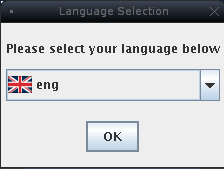
\includegraphics[width=5cm]{../image/LangChoice.png}
	\caption{Exemple de choix de langue avec IzPack}
\end{figure}
\subsubsection{Installation automatique}
A la fin de l'installation, il est possible de générer un script d'installation automatique. Ce script permet de reproduire l'installation qui vient d'être réalisée sur d'autres machines.
\begin{figure}[H]
	\centering
	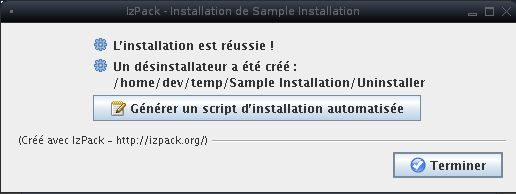
\includegraphics[width=12cm]{../image/SaveInstallXML.png}
	\caption{Fin d'installation, enregistrement du script d'installation automatisée}
\end{figure}
\subsection{Popularité du projet}
Izpack est utilisé dans de grand projets comme Jboss, Xwiki, Glassfish... Des entreprises également l'utilisent pour leurs propres applications. A l'heure actuelle, les téléchargements mensuels s'élèvent à 25.000.
\begin{figure}[H]
	\centering
	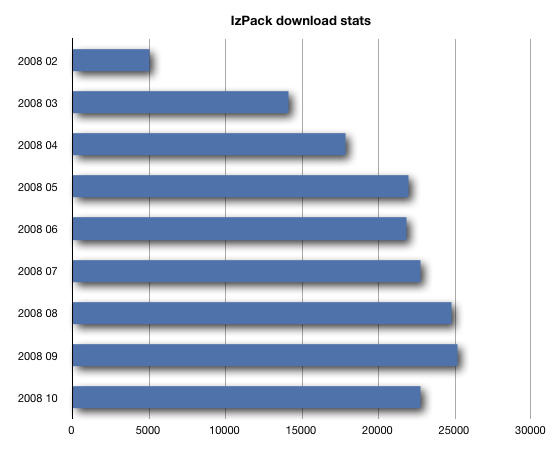
\includegraphics[width=0.6\textwidth]{../image/telechargements.png}
	\caption{Statistiques de téléchargements}
\end{figure}
 %---------------------------------------------------------
\section{Architecture}
\subsection{Architecture globale}
Globalement, Izpack possède 2 composants, le compilateur qui va gérer la création de l'installeur et l'installeur lui-même.
\subsection{Compilateur}
Le compilateur se charge de packager l'ensemble des fichiers nécessaires dans un seul fichier jar.
Ces fichiers comprennent l'application en elle-même et les fichiers nécessaires lors de l'installation. 
Selon la description de l'installation, il va incorporer les panels nécessaires à celle-ci.
Cette partie est utilisée par le développeur qui souhaite créer un installeur.
\subsection{Installeur}
La partie installation concerne toute la logique et la présentation du processus d'installation. Cette partie sera exécuter par un utilisateur souhaitant installer le logiciel.
\subsection{Processus d'installation}
Dans un premier temps, le compilateur va compiler l'application.



\begin{figure}[H]
	\centering
	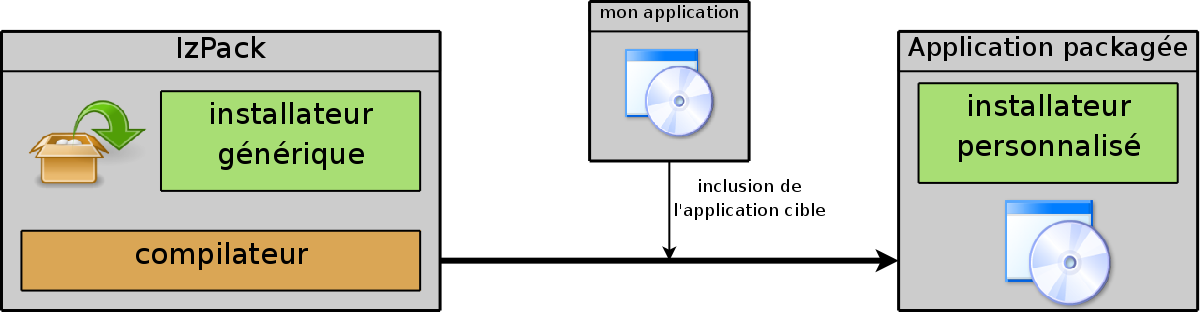
\includegraphics[width=0.8\textwidth]{../image/partie_compil.png}
	\caption{Phase de compilation}
\end{figure}
L'installateur généré comprend l'application en elle-même et toute la partie installation nécessaire et adaptée aux besoins de l'application.
Cette application est alors prête à être déployée sur une autre machine.
\begin{figure}[H]
	\centering
	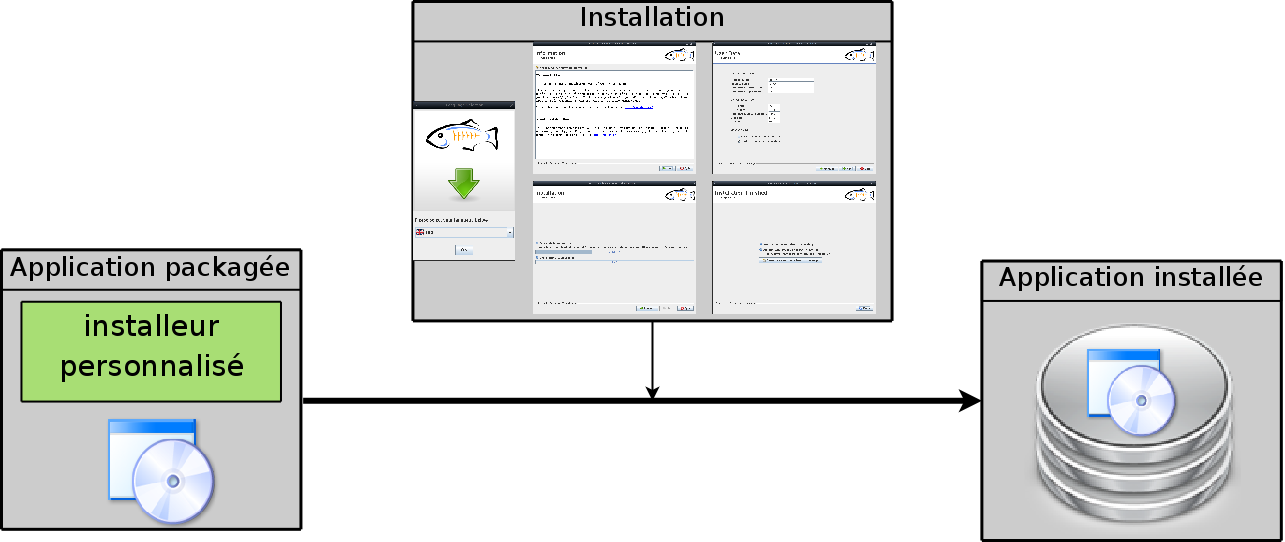
\includegraphics[width=0.8\textwidth]{../image/partie_install.png}
	\caption{Phase d'installation}
\end{figure}
Le processus d'installation est géré par la partie installeur de Izpack. Cette phase va permettre de déployer l'application sur toutes les machines nécessaires.

\subsubsection{Exemples de panels}
Il existe de nombreux types de panels : des panel pour accueillir l'utilisateur et lui afficher des informations (HelloPanel et HTMLInfoPanel), d'autres pour demander à l'utilisateur des informations (UserInputPanel), etc...
Il existe aussi des panels plus spécialisés. Ainsi, CompilePanel permet de compiler du code java et ProcessPanel permet de lancer des programmes après l'installation.

% screenshot de panels si on a du temps / de la place
%---------------------------------------------------------
\section{Exemples d'installation}
Des exemples complets existent, par exemple l'installeur de IzPack, de Glassfish, de PerfSonar... 
Pour illustrer simplement l'utilisation de IzPack, utilisons plutôt le petit exemple fourni avec le code de l'application.
\subsection{Description du xml}
Ce xml (install.xml) décrit complètement l'installation.
Une balise \verb|info| permet de définir les informations concernant l'application : 
\begin{lstlisting}[language=xml]
<info>
	<appname>Sample Installation</appname>
	<appversion>1.4 beta 666</appversion>
	...
</info>
\end{lstlisting}
Une autre balise, \verb|guipref| permet de définir quelques propriétés de la fenêtre de l'installeur :
\begin{lstlisting}[language=xml]
<guiprefs width="640" height="480" resizable="yes"/>
\end{lstlisting}
Les langues sont définies par la balise \verb|locale| :
\begin{lstlisting}
<locale>
	<langpack iso3="eng"/>
	<langpack iso3="fra"/>
</locale>
\end{lstlisting}
Des fichiers externes nécessaires à l'installation peuvent être définis par la balise \verb|resources| :
\begin{lstlisting}[language=xml]
<resources>
	<res id="LicencePanel.licence" src="Licence.txt"/>
</resources>
\end{lstlisting}
Les panels visibles par l'utilisateur sont décrits dans la balise \verb|panels| :
\begin{lstlisting}[language=xml]
<panels>
	<panel classname="HelloPanel"/>
	...
	<panel classname="FinishPanel"/>
</panels>
\end{lstlisting}
Enfin la balise \verb|packs| contient la description des packs (les différentes parties, optionnelles ou non, de l'application) à installer.
\begin{lstlisting}[language=xml]
<packs>
	<pack name="Base" required="yes">
		<description>The base files</description>
		<file src="Readme.txt" targetdir="$INSTALL_PATH"/>
		...
	</pack>
	<pack name="Docs" required="no">
		...
	</pack>
	...
</packs>
\end{lstlisting}
Bien sûr d'autres options existent, mais celles présentées ici suffisent à créer notre installeur.
Les fichiers référencés doivent être présents dans le chemin indiqué par le xml lors de la compilation.
\subsection{Génération du jar}
Pour générer notre installeur, il suffit de lancer la commande suivante : (l'exécutable \verb|compile| provient de IzPack)
\begin{verbatim}
$ compile install.xml
.::  IzPack - Version 4.1.0 ::.

< compiler spécifications version: 1.0 >

- Copyright (c) 2001-2008 Julien Ponge
- Visit http://izpack.org/ for the latest releases
- Released under the terms of the Apache Software License version 2.0.

-> Processing  : install.xml
-> Output      : install.jar
-> Base path   : .
-> Kind        : standard
-> Compression : default
-> Compr. level: -1
-> IzPack home : .

...

Build time: Tue Mar 10 16:50:27 CET 2009
\end{verbatim}
Cette exécution va produire un fichier install.jar : notre installeur.
\subsection{Installation}
Il suffit désormais de lancer le jar pour installer notre application.
\begin{figure}[H]
	\centering
	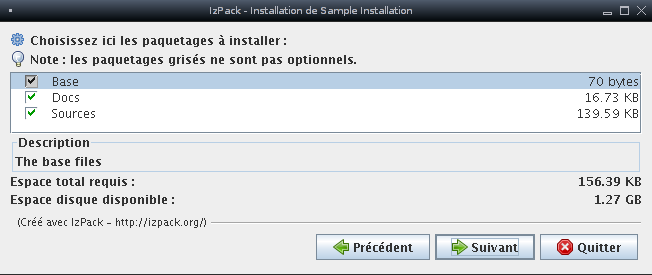
\includegraphics[width=15cm]{../image/installSample.png}
	\caption{Exemple d'installation avec IzPack}
\end{figure}
\subsection{Installation automatique}
En lançant l'installeur avec un script d'installation automatisée en paramètre, l'installation est rejouée a l'identique automatiquement.
\begin{verbatim}
$ java -jar install.jar automated.xml
[ Starting automated installation ]
[ Starting to unpack ]
[ Processing package: Base (1/3) ]
[ Processing package: Docs (2/3) ]
[ Processing package: Sources (3/3) ]
[ Unpacking finished ]
[ Writing the uninstaller data ... ]
[ Automated installation done ]
\end{verbatim}

 %---------------------------------------------------------
\section{Problèmes actuels}
IzPack possède, comme tout logiciel, des bugs potentiels ou des améliorations à effectuer.
\subsection{Code obsolète}
Izpack a débuté en 2001. 
A cette époque, la Jdk en était à la version 1.3. Il y avait donc des fonctionnalités absentes comme la genericité. 
On trouve ainsi, encore maintenant, du code utilisant de vieilles structures de données (des tableaux d'objets ou des Vectors) ou des styles de programmation abandonnés.
\subsection{Nanoxml}
%TODO Supprimer les redites de la partie 3
Une amélioration possible concerne la gestion des fichiers XML, qui ont une grande importance dans IzPack.
L'absence de processeur XML intégré à la JRE 1.3 a forcé l'utilisation d'une librairie externe pour traiter les XML.
IzPack se base donc sur une librqirie externe; nanoXML.
Cette librairie n'est malheureusement plus mise à jour (la dernière mise à jour date de 2003) et possède encore quelques bugs.
De plus, les versions récentes de l'environnement java (JRE) possèdent de base tout ce qu'il faut pour gérer le xml.
Se débarrasser de la dépendance à nanoXML et se reposer uniquement sur la JRE permettrait donc non seulement de rendre la gestion des XML plus sûre et robuste, mais également de diminuer la taille des installeurs générés.
